%%%%%%%%%%%%%%%%%%%%%%%%%%%%%%%%%%%%%%%%%
% University/School Laboratory Report
% LaTeX Template
% Version 3.1 (25/3/14)
%
% This template has been downloaded from:
% http://www.LaTeXTemplates.com
%
% Original author:
% Linux and Unix Users Group at Virginia Tech Wiki 
% (https://vtluug.org/wiki/Example_LaTeX_chem_lab_report)
%
% License:
% CC BY-NC-SA 3.0 (http://creativecommons.org/licenses/by-nc-sa/3.0/)
%
%%%%%%%%%%%%%%%%%%%%%%%%%%%%%%%%%%%%%%%%%

%----------------------------------------------------------------------------------------
%	PACKAGES AND DOCUMENT CONFIGURATIONS
%----------------------------------------------------------------------------------------

\documentclass[12pt]{article}

\usepackage[hmargin=3cm, vmargin=2cm]{geometry} % set margins

\usepackage{graphicx} % Required for the inclusion of images
\usepackage{natbib} % Required to change bibliography style to APA
\usepackage{amsmath} % Required for some math elements 
\usepackage[utf8]{inputenc} % Use UTF-8
\usepackage{float}

\setlength\parindent{0pt} % Removes all indentation from paragraphs

\graphicspath{{images/}} % Define graphics path

\renewcommand{\labelenumi}{\alph{enumi}.} % Make numbering in the enumerate environment by letter rather than number (e.g. section 6)

\renewcommand{\baselinestretch}{1.5} % set line spacing

\usepackage{times} % Uncomment to use the Times New Roman font

%----------------------------------------------------------------------------------------
%	DOCUMENT INFORMATION
%----------------------------------------------------------------------------------------

\title{Data Analysis and Knowledge Discovery \\ Exercise Work 1} % Title

\author{Tatu Seppä-Lassila} % Author name

\date{\today} % Date for the report

\begin{document}

\maketitle % Insert the title, author and date

%----------------------------------------------------------------------------------------
%	SECTIONS
%----------------------------------------------------------------------------------------
 
\section{Task 1: Histograms}

Histograms were plotted using python and matplotlib. Freedman-Diaconis rule, Sturges' rule and Square-root choice was used to calculate the number of bins in the histograms. These three histograms were plotted for all of the attributes. However, only plots for alcohol are shown in this documents to demonstrate the results. 

% Histogram, Freedman Diaconis
\begin{figure}[H]
    \centering
    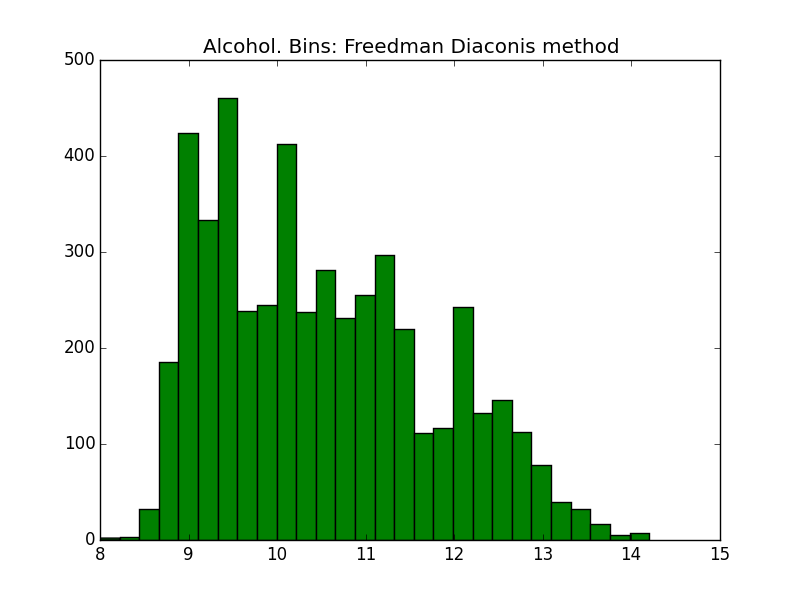
\includegraphics[width=0.8\textwidth]{alcohol_fdr}
    \caption{Histogram of alcohol attribute. Number of bins selected with Freedman-Diaconis rule.}
    \label{fig:histogram_fdr}
\end{figure}
% End of picture

% Histogram, Freedman Diaconis
\begin{figure}[H]
    \centering
    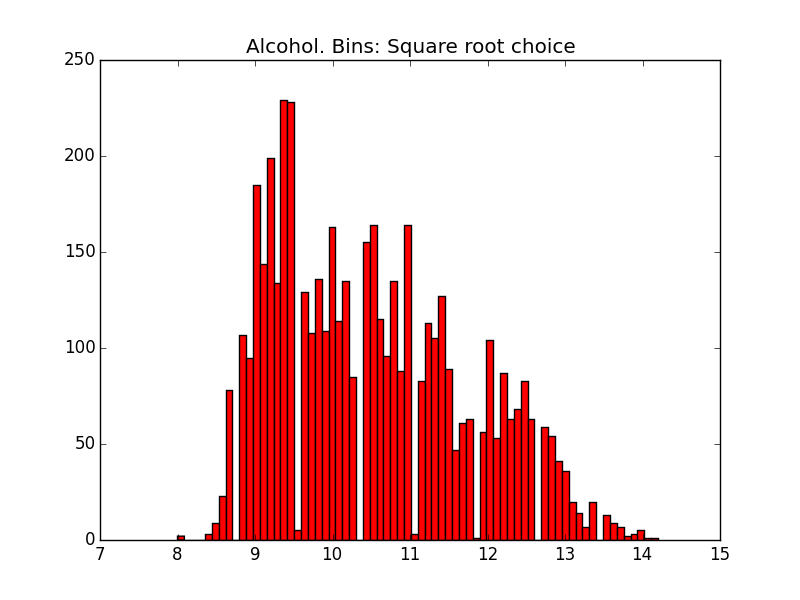
\includegraphics[width=0.8\textwidth]{alcohol_src}
    \caption{Histogram of alcohol attribute. Number of bins selected with Square-root choice.}
    \label{fig:histogram_src}
\end{figure}
% End of picture

% Histogram, Sturges' rule
\begin{figure}[H]
    \centering
    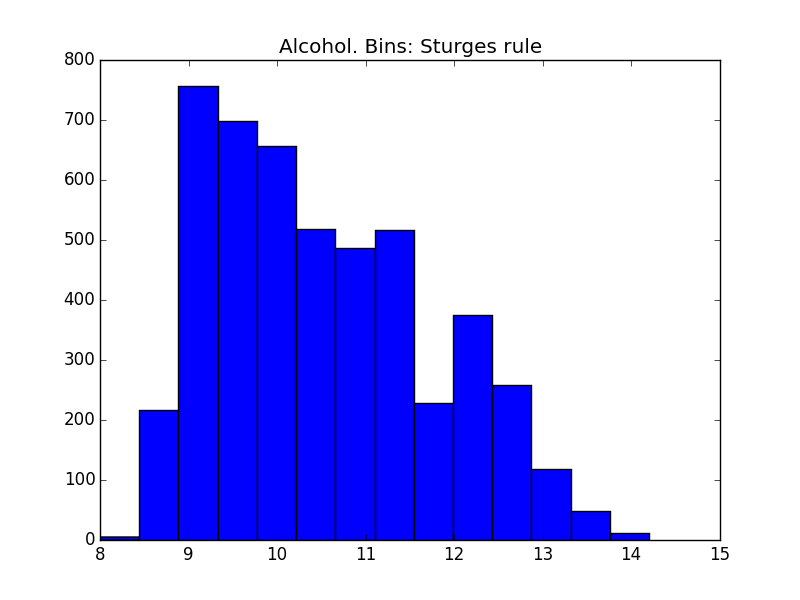
\includegraphics[width=0.8\textwidth]{alcohol_sturge}
    \caption{Histogram of alcohol attribute. Number of bins selected with Sturges' rule.}
    \label{fig:histogram_sturge}
\end{figure}
% End of picture

Figures \ref{fig:histogram_fdr}, \ref{fig:histogram_src}, \ref{fig:histogram_sturge} show the plotted histograms for alcohol attribute. Square-root choice produced 70 bins with this dataset. Respectively, Freedman-Diaconis rule produced 28 bins and Sturges' 14 bins. Histograms with lower number of bins show that majority of samples have alcohol around 10. Figure \ref{fig:histogram_src} shows that higher number of bins reveal that some tenths have very low number of samples, even though the next tenth has 50 or more samples.%

\section{Task 2: Scatter Plots and Parallel Coordinates Representation}

\section{Task 3: Principal Component Analysis}

\section{Task 4: 2D Multidimensional Scaling}

\section{Task 5: Pearson and Kendall's Tau Correlation Tables}


\end{document}